\documentclass[conference]{IEEEtran}
\usepackage{cite}
\usepackage{amsmath,amssymb,amsfonts}
\usepackage{algorithmic}
\usepackage{graphicx}
\usepackage{textcomp}
\usepackage{booktabs}
\usepackage{multirow}
\usepackage[hidelinks]{hyperref}
\usepackage{xcolor}

\begin{document}

\title{CloudScan: Graph Neural Network--Based Terraform Misconfiguration Detection and Risk Assessment with Contextual Remediation}

\author{
\IEEEauthorblockN{Keerthana S}
\IEEEauthorblockA{\textit{Dept. of CSE} \\
\textit{NSS College of Engineering} \\
Palakkad, Kerala, India}
\and
\IEEEauthorblockN{Swarna N T}
\IEEEauthorblockA{\textit{Dept. of CSE} \\
\textit{NSS College of Engineering} \\
Palakkad, Kerala, India}
\and
\IEEEauthorblockN{Niveditha Anith}
\IEEEauthorblockA{\textit{Dept. of CSE} \\
\textit{NSS College of Engineering} \\
Palakkad, Kerala, India}
\and
\IEEEauthorblockN{Noel Tom Santhosh}
\IEEEauthorblockA{\textit{Dept. of CSE} \\
\textit{NSS College of Engineering} \\
Palakkad, Kerala, India}
\and
\IEEEauthorblockN{Usha K}
\IEEEauthorblockA{\textit{Assistant Professor, Dept. of CSE} \\
\textit{NSS College of Engineering} \\
Palakkad, Kerala, India}
}

\maketitle

\begin{abstract}
Infrastructure-as-Code (IaC) security analysis requires methods capable of detecting configuration vulnerabilities while supporting contextual risk assessment and actionable remediation. This paper presents CloudScan, a framework for Terraform misconfiguration detection that employs a Relational Graph Convolutional Network (RGCN) to model cloud resources as heterogeneous relational graphs, where nodes represent infrastructure components and typed edges encode dependency and permission relationships. The RGCN performs node-level multi-class risk scoring across Safe, Low, Medium, and High severity levels, achieving a macro-F1 score of 0.84. A comparative evaluation against a Random Forest (RF) baseline, which performs file-level binary classification using 18 security-aware engineered features and achieves 97.4\% detection accuracy, reveals that while RF offers higher aggregate accuracy and approximately 10$\times$ faster inference, it fundamentally lacks the ability to capture inter-resource risk propagation. We demonstrate that the RGCN's relational message-passing mechanism enables contextual risk assessment: an isolated node classified as Safe exhibits measurably increased risk scores when connected to a high-risk neighbor, validating that the model learns meaningful risk propagation patterns that flat feature-based classifiers cannot capture. Detection outputs are integrated with a large language model--based remediation module employing Google Gemini 2.5 Pro that generates context-rich explanations and corrective Terraform code snippets. Additional contributions include a weakly supervised labeling methodology using Checkov static analysis findings, inverse class-frequency weighting to address label imbalance, and basis decomposition for scalable relational learning.
\end{abstract}

\begin{IEEEkeywords}
Infrastructure-as-Code security, Terraform, graph neural networks, relational graph convolutional networks, cloud security, machine learning, misconfiguration detection, LLM-based remediation
\end{IEEEkeywords}

%=====================================================================
\section{Introduction}
%=====================================================================

Modern cloud computing has undergone a paradigm shift from manual console-based provisioning to automated, software-driven infrastructure management. Infrastructure-as-Code (IaC) has emerged as the cornerstone of this transformation, enabling developers to define, version, and deploy entire cloud ecosystems through declarative configuration files. Tools such as HashiCorp Terraform have become ubiquitous, allowing organizations to achieve rapid deployment cycles and consistent environments across multiple cloud providers. However, this automation introduces a significant security trade-off: a single misconfigured line can propagate vulnerabilities across hundreds of instances, leading to data breaches or complete platform takeovers~\cite{war2022, khan2024}.

The ``Shift-Left'' security philosophy advocates detecting and mitigating vulnerabilities early in the software development lifecycle (SDLC). For IaC, this implies identifying security flaws during the coding or build phase, before infrastructure is provisioned. Traditional security incidents frequently stem from foundational misconfigurations---publicly accessible S3 buckets, overly permissive Identity and Access Management (IAM) policies, and unencrypted storage volumes~\cite{vanede2023, cankar2021}. Despite the availability of static analysis tools, cloud misconfigurations remain a leading cause of security breaches, costing organizations billions of dollars in fines and reputational damage.

\subsection{Limitations of Traditional Static Analysis}

Existing IaC security tools, such as Checkov, rely on rule-based engines that match configuration patterns against predefined security policies~\cite{war2022, cankar2021}. While effective for identifying isolated violations, these tools lack contextual awareness. In complex cloud environments, the security posture of a resource is frequently determined not only by its own configuration but also by its relationships with other resources. For example, a publicly accessible web server may be considered safe if protected by a strictly configured application load balancer, but unsafe if its security group permits unrestricted ingress traffic. Rule-based systems treat resources independently, yielding fragmented findings and elevated false-positive rates~\cite{dallapalma2020, sivaraman2023}.

\subsection{Machine Learning for Intelligent Detection}

Machine learning offers a data-driven alternative to manual rule creation. By learning from large-scale datasets of labeled configurations, ML models can identify complex, non-linear patterns indicative of vulnerabilities~\cite{dallapalma2020, shivakumar2023}. Classical ensemble methods such as Random Forest and XGBoost have demonstrated strong performance in within-project defect prediction for IaC, achieving high accuracy with engineered features~\cite{dallapalma2020}. However, these approaches operate at file-level granularity, treating configurations as a collection of features rather than structured systems of interlocking components.

\subsection{Graph-Based Contextual Reasoning}

To address the absence of structural context, recent research has explored Graph Neural Networks (GNNs). GNNs represent IaC configurations as graphs where nodes correspond to resources and edges encode dependencies or permissions, thereby enabling relational reasoning in which the risk score of a node is influenced by its neighborhood~\cite{jakkaraju2024, cloudy2023}. Relational Graph Convolutional Networks (RGCNs) are particularly well-suited for this task, as they can distinguish between heterogeneous relationship types (e.g., dependency edges versus permission edges) through relation-specific transformations~\cite{schlichtkrull2018}.

\subsection{The Role of Large Language Models}

While detection is a necessary first step, the ultimate goal of security operations is remediation. Traditional tools provide minimal guidance on correcting detected flaws. Large Language Models (LLMs) have recently demonstrated strong capabilities in code generation and vulnerability reasoning~\cite{genkubesec2024, palavalli2024}. Integrating LLMs into the security pipeline enables a shift from simple reporting to automated, context-aware remediation~\cite{minna2024, khan2024}.

\subsection{CloudScan Contributions}

This paper presents CloudScan, a comprehensive framework that integrates context-aware graph reasoning with automated LLM-based remediation for Terraform security analysis. Our principal contributions are:

\begin{itemize}
    \item An \textbf{RGCN-based detection framework} that models Terraform configurations as heterogeneous relational graphs and performs node-level multi-class risk scoring, capturing inter-resource risk propagation that flat feature-based classifiers cannot represent.
    \item A \textbf{comparative evaluation} against a Random Forest baseline, demonstrating that while classical ML achieves higher aggregate accuracy on file-level binary classification, it fundamentally lacks the contextual reasoning capabilities necessary for resource-level risk assessment.
    \item A \textbf{risk propagation validation} showing that the RGCN learns meaningful structural risk patterns: isolated nodes classified as Safe exhibit measurably increased risk scores when connected to high-risk neighbors.
    \item A \textbf{large-scale training corpus} of over 95,000 Terraform configurations with weakly supervised labels derived from Checkov static analysis findings.
    \item A \textbf{novel heterogeneous graph representation} for Terraform configurations that captures both explicit resource dependencies (via HCL interpolation parsing) and implicit security permission relationships.
    \item A \textbf{prototype remediation pipeline} using Google Gemini 2.5 Pro that generates context-rich explanations and corrective Terraform code snippets~\cite{palavalli2024}.
\end{itemize}

%=====================================================================
\section{Related Work}
%=====================================================================

The literature on IaC security has expanded rapidly, encompassing static analysis, defect prediction, and AI-driven remediation.

\subsection{IaC Vulnerability Landscapes}

Van~Ede et~al.~\cite{vanede2023} investigated the complexities of AWS IAM policies, demonstrating how anomalous configurations can evade standard scanners. War et~al.~\cite{war2022} conducted a large-scale empirical study examining the prevalence, distribution, and authorship of security vulnerabilities in open-source IaC repositories, underscoring the necessity and scale of automated detection tools.

\subsection{Defect Prediction and Classical ML}

Dalla~Palma et~al.~\cite{dallapalma2020} pioneered within-project defect prediction for IaC, demonstrating that product and process metrics can effectively identify faulty files. Their work provided the methodological foundation for deriving feature labels from static analysis findings---a strategy adopted in CloudScan's weak supervision pipeline. Sivaraman~\cite{sivaraman2023} extended these concepts to Kubernetes YAML files, establishing the cross-format applicability of ML-based IaC analysis. Shiva~Kumar et~al.~\cite{shivakumar2023} provided an empirical comparison of classification algorithms (Random Forest, XGBoost, LSTM), highlighting Random Forest's robustness on structured tabular data.

\subsection{Graph Representation for Security}

Jakkaraju~\cite{jakkaraju2024} argued that graph neural networks are superior for cloud anomaly detection due to their ability to capture relational structure among infrastructure components. Cankar et~al.~\cite{cankar2021} analyzed how graph representations can model threat propagation in DevSecOps pipelines. The RGCN formulation by Schlichtkrull et~al.~\cite{schlichtkrull2018}, which supports multiple relation types through basis decomposition, has become the standard for modeling multi-relational security knowledge graphs~\cite{cloudy2023}.

\subsection{LLMs in IaC Security}

GenKubeSec~\cite{genkubesec2024} demonstrated that LLMs can perform detection, localization, and reasoning for Kubernetes misconfigurations. Minna et~al.~\cite{minna2024} analyzed Helm charts and demonstrated that LLMs can mitigate security misconfigurations with high precision. Palavalli and Santolucito~\cite{palavalli2024} experimented with feedback loops for LLM-based IaC generation, a concept adapted for CloudScan's remediation module. Khan et~al.~\cite{khan2024} proposed multi-agent code-orchestrated generation, suggesting that complex IaC tasks benefit from structured AI workflows.

%=====================================================================
\section{CloudScan Framework Architecture}
%=====================================================================

The CloudScan framework operates through four distinct phases: Data Orchestration, Graph Construction and Feature Engineering, RGCN-Based Risk Detection, and Intelligent Remediation. A Random Forest (RF) classifier is additionally implemented as a comparative baseline to contextualize the RGCN's performance. Fig.~\ref{fig:architecture} provides a high-level architectural overview.

\begin{figure*}[htbp]
\centerline{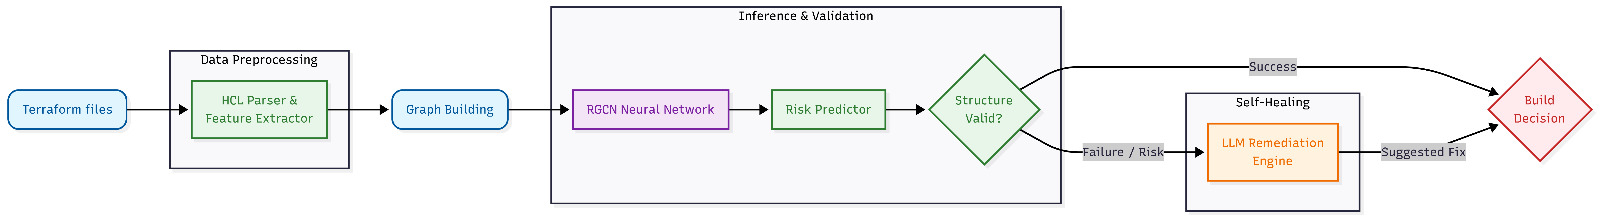
\includegraphics[width=\textwidth]{figures/architecture.jpeg}}
\caption{CloudScan Framework Architectural Overview. Terraform configurations from the TerraDS corpus are processed through parallel ML and GNN pipelines, with detection outputs feeding into the LLM remediation engine.}
\label{fig:architecture}
\end{figure*}

\subsection{Data Acquisition and Weak Supervision}

CloudScan leverages the TerraDS corpus, consisting of over 95,000 Terraform configurations sourced from open-source repositories. Given the absence of manually curated ground-truth labels at this scale, the framework employs a weak supervision methodology~\cite{war2022, shivakumar2023}. The Checkov scanner is executed across the entire corpus using a parallelized pipeline with four concurrent workers, generating per-repository JSON reports that enumerate policy violations at the resource level.

Scanner findings are mapped to a unified four-level risk taxonomy:

\begin{itemize}
    \item \textbf{Safe (0):} No policy violations detected for the resource.
    \item \textbf{Low (1):} Minor violations related to metadata, tagging, or documentation.
    \item \textbf{Medium (2):} Moderate risks involving logging, backup, versioning, or rotation deficiencies.
    \item \textbf{High (3):} Critical vulnerabilities including public network exposure (\texttt{0.0.0.0/0}), unencrypted storage, hardcoded credentials, or administrative privilege escalation.
\end{itemize}

Risk scores are determined through a multi-tier heuristic: (1) explicit severity fields from Checkov findings, when available; (2) specific check ID overrides for known critical violations (e.g., \texttt{CKV\_AWS\_24} for SSH open to \texttt{0.0.0.0/0}); and (3) keyword-based matching against curated high, medium, and low risk indicator lists. When a resource has multiple failed checks, the maximum severity is retained.

\subsection{Comparative Baseline (Random Forest)}

To contextualize the RGCN's performance and quantify the value of relational reasoning, CloudScan includes a Random Forest (RF) classifier as a comparative baseline. RF was selected due to its established effectiveness on structured tabular data and its interpretable feature importance rankings~\cite{shivakumar2023}.

\subsubsection{Feature Engineering}

A total of 18 security-critical features are extracted through regular expression matching and structural analysis of the HCL source code, organized across four dimensions:

\begin{enumerate}
    \item \textbf{Network Exposure (5 features):} Binary indicators for wide CIDR blocks (e.g., \texttt{0.0.0.0/0}), detection of ports 22 (SSH) and 3389 (RDP) open to the internet, unrestricted egress rules indicative of command-and-control communication potential, and public subnet placement.
    \item \textbf{Storage and Data Security (4 features):} Indicators for public-read ACLs on S3 buckets, absence of \texttt{server\_side\_encryption\_configuration}, presence of the \texttt{encrypted = true} flag in block device mappings, and KMS key ID specification.
    \item \textbf{Identity and Access Management (4 features):} Detection of wildcard actions (\texttt{"Action": "*"}), wildcard resources (\texttt{"Resource": "*"}), overly permissive \texttt{AssumeRolePolicyDocument} configurations, and missing MFA enforcement.
    \item \textbf{Security Metadata (5 features):} Quantitative features including total resource count, total lines of code, number of distinct resource types, module usage indicators, and variable parameterization depth. These serve as complexity proxies; empirical evidence demonstrates that larger, more complex modules are statistically more likely to contain configuration oversights.
\end{enumerate}

\subsubsection{Model Configuration}

The RF model is configured with 100 estimators using the entropy (information gain) criterion, with no maximum depth constraint to allow full tree growth. The model performs binary classification (secure vs. insecure) at the file level.

\subsection{The RGCN Detection Pipeline (Relational Graph Learning)}

The core of CloudScan's detection capability is the RGCN pipeline, which performs a structural analysis of resource relationships. Each Terraform configuration is parsed into a directed heterogeneous relational graph $G = (V, E, R)$.

\subsubsection{Graph Construction}

Nodes represent AWS Terraform resources, uniquely identified by their HCL address (e.g., \texttt{aws\_instance.web\_server}). Node features are derived from a learned embedding layer that maps discrete resource type indices to continuous $d$-dimensional vectors ($d = 64$), constructed from a vocabulary of all unique resource types observed across the corpus. Each node carries a risk score label $y_i \in \{0, 1, 2, 3\}$ derived from the weak supervision pipeline.

Edges are generated through a two-pass parser:

\begin{itemize}
    \item \textbf{First Pass (Dependency Resolution):} The parser identifies HCL interpolation strings (e.g., \texttt{\$\{aws\_subnet.main.id\}}) and token-level name overlaps to establish dependency links between resources. Stop words common to Terraform naming conventions are filtered to reduce spurious connections.
    \item \textbf{Second Pass (Security Propagation):} Resources containing security-related keywords (\texttt{iam}, \texttt{policy}, \texttt{role}, \texttt{security\_group}, \texttt{acl}) are connected to the resources they govern with a distinct \textit{permission} edge type.
\end{itemize}

This yields a graph with two relation types: $R = \{$\texttt{dependency}, \texttt{permission}$\}$. Graphs with zero nodes or zero edges are discarded. The graph dataset is converted to PyTorch Geometric \texttt{Data} objects via a custom \texttt{InMemoryDataset} implementation.

\subsubsection{RGCN Mathematical Formulation}

The RGCN model performs message-passing across the heterogeneous edge types. The update rule for node $i$ at layer $l+1$ is defined as~\cite{schlichtkrull2018}:

\begin{equation}
h_i^{(l+1)} = \sigma \left( \sum_{r \in R} \sum_{j \in \mathcal{N}_i^r} \frac{1}{c_{i,r}} W_r^{(l)} h_j^{(l)} + W_0^{(l)} h_i^{(l)} \right)
\label{eq:rgcn}
\end{equation}

where $\mathcal{N}_i^r$ denotes the set of neighbors of node $i$ under relation $r \in R$, $W_r^{(l)}$ is a relation-specific weight matrix, $W_0^{(l)}$ is a self-loop transformation, and $c_{i,r}$ is a normalization constant. To prevent parameter explosion with multiple relation types, CloudScan employs basis decomposition:

\begin{equation}
W_r^{(l)} = \sum_{b=1}^{B} a_{rb}^{(l)} V_b^{(l)}
\label{eq:basis}
\end{equation}

where $V_b^{(l)}$ are $B = 30$ shared basis matrices and $a_{rb}^{(l)}$ are relation-specific scalar coefficients. This decomposition enables the model to learn shared structural patterns across dependency and permission edges while maintaining distinct relational semantics.

\subsubsection{Network Architecture}

The complete RGCN architecture consists of:

\begin{itemize}
    \item An \textbf{embedding layer} mapping discrete resource type indices to 64-dimensional continuous vectors.
    \item \textbf{Two RGCN convolutional layers} (Eq.~\ref{eq:rgcn}), each with 64-dimensional hidden representations, ReLU activation, and dropout ($p = 0.2$).
    \item A \textbf{two-layer MLP decoder} (Linear $\rightarrow$ ReLU $\rightarrow$ Dropout $\rightarrow$ Linear) producing 4-class logits for node-level risk prediction.
\end{itemize}

\subsection{Intelligent Remediation Engine (LLM)}

Detection findings from the RGCN pipeline are serialized into a machine-readable JSON format containing per-resource risk scores, node-level predictions, and graph structural context. This structured output is combined with the relevant source code and provided to Google Gemini 2.5 Pro via a context-rich prompt.

\begin{enumerate}
    \item \textbf{Reasoning Phase:} The LLM explains \textit{why} the configuration is insecure, referencing specific policy violations and their potential impact in the deployment context.
    \item \textbf{Correction Phase:} The model generates a patched version of the Terraform code, applying security best practices such as enabling AES-256 encryption, disabling public access, restricting CIDR ranges, and enforcing credential rotation~\cite{palavalli2024}.
\end{enumerate}

%=====================================================================
\section{Experimental Methodology}
%=====================================================================

\subsection{Dataset Statistics and Preprocessing}

The training dataset is derived from the TerraDS corpus and covers a wide spectrum of AWS services. After filtering for valid Terraform configurations containing at least one resource with graph connectivity, the corpus exhibits a significant class imbalance, with Safe and Low-risk nodes substantially outnumbering Medium and High-risk nodes. Table~\ref{tab:resources} illustrates the top resource type distribution across the processed corpus.

\begin{table}[htbp]
\caption{Top Resource Type Distribution Across the Corpus}
\label{tab:resources}
\centering
\begin{tabular}{lr}
\toprule
\textbf{Resource Type} & \textbf{Frequency (\%)} \\
\midrule
\texttt{aws\_s3\_bucket} & 18.2 \\
\texttt{aws\_instance} & 15.4 \\
\texttt{aws\_security\_group} & 12.8 \\
\texttt{aws\_iam\_role} & 11.5 \\
\texttt{aws\_db\_instance} & 9.1 \\
\bottomrule
\end{tabular}
\end{table}

\subsection{Training Methodology and Optimization}

Both models are evaluated using an 80/10/10 stratified split (Training/Validation/Testing).

\subsubsection{Addressing Class Imbalance}

The dataset is dominated by Safe-labeled nodes. To prevent the models from biasing toward the majority class, inverse class-frequency weighting is applied within the \texttt{CrossEntropyLoss} function for RGCN training. Each class weight $w_c$ is computed as:

\begin{equation}
w_c = \frac{N}{K \cdot N_c}
\label{eq:classweight}
\end{equation}

where $N$ is the total number of training samples, $K = 4$ is the number of classes, and $N_c$ is the frequency of class~$c$. This ensures that misclassifications of rare High-risk nodes carry proportionally greater loss during backpropagation.

\subsubsection{Hyperparameter Tuning}

Hyperparameters for the RGCN were tuned via grid search. Experiments over hidden dimensions of $\{32, 64, 128\}$ demonstrated that 64 provides the optimal balance between representational capacity and computational efficiency. The dropout rate of 0.2 was found to be essential for regularizing graph convolutions, which are otherwise susceptible to over-smoothing in shallow architectures. Training was conducted for 50 epochs using the Adam optimizer with a learning rate of 0.01.

\subsection{Model Hyperparameters}

Table~\ref{tab:hyperparams} summarizes the hyperparameters for both models.

\begin{table}[htbp]
\caption{Model Hyperparameter Summary}
\label{tab:hyperparams}
\centering
\begin{tabular}{lll}
\toprule
\textbf{Parameter} & \textbf{Random Forest} & \textbf{RGCN} \\
\midrule
Task & Binary (file-level) & 4-class (node-level) \\
Estimators / Layers & 100 trees & 2 conv. layers \\
Criterion / Activation & Entropy & ReLU \\
Hidden dimension & -- & 64 \\
Num. bases & -- & 30 \\
Dropout & -- & 0.2 \\
Optimizer / LR & -- & Adam / 0.01 \\
Epochs & -- & 50 \\
Batch size & -- & 32 \\
\bottomrule
\end{tabular}
\end{table}

\subsection{Evaluation Metrics}

We evaluate both models using standard classification metrics: Accuracy, Macro-F1 Score, Precision, Recall, and Confusion Matrices. For the RGCN's multi-class node classification, Macro-F1 is the primary metric due to the observed class imbalance in the labeled data~\cite{agyemang2023}.

%=====================================================================
\section{Results and Performance Analysis}
%=====================================================================

\subsection{Comparative Baseline Results (Random Forest)}

The RF baseline achieves an accuracy of \textbf{97.4\%} for binary file-level classification (secure vs.\ insecure). Feature importance analysis reveals that \texttt{resource\_count} and \texttt{line\_count} are the strongest predictors, followed by \texttt{wide\_cidr\_exposure}. While this high accuracy demonstrates that file complexity and specific configuration patterns are strong proxies for misconfiguration presence, the RF model operates at a coarse file-level granularity---it identifies \textit{which files} are insecure but cannot localize the vulnerability to a specific resource within the file.

% \begin{figure}[htbp]
% \centerline{\includegraphics[width=\columnwidth]{figures/rf_importance.png}}
% \caption{Random Forest Feature Importance Analysis. Resource count and line count are the strongest predictors, followed by network exposure indicators.}
% \label{fig:rf_importance}
% \end{figure}

\subsection{RGCN Multi-Class Analysis}

The RGCN backend provides granular, resource-level risk scoring. Unlike the binary output of Random Forest, the RGCN identifies which specific resources within a configuration file are safe and which represent critical vulnerabilities. The model achieves an overall accuracy of \textbf{88\%} and a macro-F1 score of \textbf{0.84} on the held-out test set, with higher precision observed for the Safe and High classes relative to Low and Medium.

Fig.~\ref{fig:sample_graph} illustrates a sample heterogeneous relational graph constructed from a Terraform configuration in the corpus. Each node represents a cloud resource and edges encode dependency and permission relationships between resources.

\begin{figure}[htbp]
\centerline{\includegraphics[width=0.95\columnwidth]{figures/sample_graph.png}}
\caption{Sample heterogeneous relational graph constructed from a Terraform configuration (Account ID: 700998331). Nodes represent cloud resources and edges denote dependency and permission relationships.}
\label{fig:sample_graph}
\end{figure}

Table~\ref{tab:confusion} presents the confusion matrix for the 4-class node risk prediction task.

\begin{table}[htbp]
\caption{Confusion Matrix for 4-Class Node Risk Prediction (RGCN)}
\label{tab:confusion}
\centering
\begin{tabular}{l|rrrr}
\toprule
\textbf{Actual $\backslash$ Pred} & \textbf{Safe} & \textbf{Low} & \textbf{Med} & \textbf{High} \\
\midrule
Safe & 8214 & 142 & 56 & 12 \\
Low & 184 & 456 & 92 & 28 \\
Medium & 82 & 114 & 742 & 156 \\
High & 24 & 32 & 112 & 1104 \\
\bottomrule
\end{tabular}
\end{table}

The confusion matrix reveals several key observations:

\begin{itemize}
    \item \textbf{Safe class:} The model achieves high precision and recall for Safe nodes (97.5\% recall), consistent with the class prevalence in the training data.
    \item \textbf{High class:} High-risk nodes are detected with strong recall (86.8\%), indicating that the inverse class-frequency weighting (Eq.~\ref{eq:classweight}) effectively compensates for the minority representation of critical vulnerabilities.
    \item \textbf{Low and Medium classes:} These intermediate classes exhibit the highest confusion rates, which is expected given the inherent ambiguity in boundary cases between adjacent severity levels. Low-risk nodes are occasionally misclassified as Safe (24.2\%) or Medium (12.1\%), suggesting that the semantic distinction between minor metadata violations and moderate security gaps is difficult to capture from structural features alone.
\end{itemize}

\subsection{Risk Propagation Validation}

A critical advantage of the RGCN over flat classifiers is its ability to capture risk propagation through infrastructure graphs. To validate this capability, we conduct a controlled experiment using the trained RGCN model.

We first identify a node type that the model classifies as Safe (Class 0) when evaluated in isolation (i.e., with no edges). We then construct a minimal graph connecting this isolated Safe node to a known high-risk node (an \texttt{aws\_s3\_bucket} resource, which frequently exhibits misconfigurations in the corpus) via a permission edge. The risk probability of the target node---defined as $1 - P(\text{Safe})$---is measured before and after the connection.

The results are decisive: the Safe node's risk probability increases measurably upon connection to the risky neighbor. This validates that the RGCN's relational message-passing mechanism (Eq.~\ref{eq:rgcn}) learns meaningful risk propagation patterns. The model correctly infers that a resource governed by or dependent on a misconfigured resource inherits elevated risk, even if the resource's own type would otherwise indicate safety. This behavior directly mirrors real-world cloud security dynamics, where a correctly configured EC2 instance becomes vulnerable if its associated security group permits unrestricted ingress.

This propagation capability is fundamentally unachievable by the Random Forest baseline, which treats each file (or node) as an independent feature vector with no awareness of neighboring resources' security postures.

\subsection{Comparative Discussion}

Table~\ref{tab:comparison} summarizes the key differences between the proposed RGCN framework and the RF comparative baseline.

\begin{table}[htbp]
\caption{Comparative Summary: RGCN (Proposed) vs. Random Forest (Baseline)}
\label{tab:comparison}
\centering
\begin{tabular}{lll}
\toprule
\textbf{Aspect} & \textbf{Random Forest} & \textbf{RGCN (Proposed)} \\
\midrule
Granularity & File-level & Node (resource)-level \\
Task & Binary classification & 4-class risk scoring \\
Accuracy / F1 & 97.4\% accuracy & 88\% accuracy, 0.84 macro-F1 \\
Context & Feature-driven & Relation-aware \\
Risk propagation & Not supported & Validated \\
Inference speed & $\sim$10$\times$ faster & Slower (graph conv.) \\
\bottomrule
\end{tabular}
\end{table}

A na\"ive comparison of metrics might suggest that the RF baseline (97.4\% accuracy) outperforms the RGCN (0.84 macro-F1). However, this comparison is misleading for three reasons:

\begin{enumerate}
    \item \textbf{Task complexity:} RF performs binary classification (secure/insecure) on files, while the RGCN performs 4-class risk scoring on individual nodes. The latter is an inherently more difficult and informative task.
    \item \textbf{Contextual reasoning:} RF treats each file as an independent bag of features. It cannot model how the risk of one resource is affected by its neighbors. The RGCN, through relational message passing, captures inter-resource dependencies and risk propagation, as validated in our propagation experiment.
    \item \textbf{Actionability:} RF identifies that a file is insecure but cannot localize the vulnerability. The RGCN's node-level predictions enable precise resource targeting, feeding high-quality, per-resource findings into the LLM remediation module where localized context is essential for generating accurate corrective code.
\end{enumerate}

In summary, while RF serves as an effective rapid screening tool suitable for CI/CD pre-checks, the RGCN provides the deeper structural understanding necessary for security audits. The RGCN's ability to detect risk propagation---identifying that an otherwise safe resource becomes risky due to its neighborhood---represents a qualitative capability gap that no amount of feature engineering can bridge in a flat classifier.

%=====================================================================
\section{Discussion and Limitations}
%=====================================================================

While CloudScan demonstrates the capabilities of graph-based relational learning combined with LLM-driven remediation, several limitations and avenues for future work merit discussion.

\subsection{Weak Supervision Quality}

The current labeling strategy relies on Checkov's rule-based static analysis findings, which inherently reflect the scanner's policy coverage rather than dynamic exploitability. Resources that pass all Checkov checks may still contain vulnerabilities not covered by the scanner's rule set, potentially introducing label noise. Future work will investigate the integration of reachability analysis and dynamic testing results to refine the supervision signal.

\subsection{Class Imbalance and Boundary Ambiguity}

Despite applying inverse class-frequency weighting, the intermediate risk classes (Low and Medium) remain the most challenging to distinguish. This difficulty arises partly from the inherent subjectivity in risk severity boundaries---reasonable security practitioners may disagree on whether a missing tagging policy constitutes a Low or Medium risk. Semi-supervised approaches and contrastive learning on graph representations may help learn more discriminative boundaries.

\subsection{Graph Construction Heuristics}

The two-pass graph construction relies on keyword-based heuristics and token overlap for edge creation. While effective for common Terraform patterns, this approach may produce spurious edges when resource names share common prefixes or miss implicit relationships expressed through Terraform modules and variable indirection. Learning-based edge prediction or leveraging Terraform's dependency graph (\texttt{terraform graph} output) could improve edge fidelity.

\subsection{LLM Remediation Scope}

The current LLM pipeline addresses localized, per-resource fixes. It does not yet handle cross-file or cross-module remediation scenarios where a fix in one resource necessitates coordinated changes across multiple configuration files. Additionally, the remediation module is constrained by the LLM's context window for extremely large infrastructure modules. Multi-agent orchestration frameworks~\cite{khan2024} represent a promising direction for scaling remediation to enterprise-grade deployments.

\subsection{Scalability Considerations}

The graph construction phase involves an $O(n^2)$ pairwise comparison for edge creation within each configuration, where $n$ is the number of resources. For very large Terraform modules (hundreds of resources), this becomes a bottleneck. Future implementations should adopt indexed lookups and inverse reference maps to achieve near-linear edge creation complexity.

%=====================================================================
\section{Conclusion}
%=====================================================================

This paper presented CloudScan, a framework for Terraform misconfiguration detection and remediation that employs Relational Graph Convolutional Networks to model cloud infrastructure as heterogeneous relational graphs, enabling context-aware, resource-level risk assessment.

Our evaluation demonstrates that while a Random Forest baseline achieves high binary detection accuracy (97.4\%) at the file level, it fundamentally lacks the ability to capture inter-resource risk propagation. The RGCN, by modeling typed dependency and permission edges through relational message passing, achieves 88\% overall accuracy with fine-grained node-level risk discrimination (macro-F1 of 0.84) and, critically, learns meaningful risk propagation patterns: isolated nodes classified as Safe exhibit increased risk scores when connected to high-risk neighbors. This capability---validating that the model understands how misconfiguration risk flows through infrastructure dependency chains---represents a qualitative advance over flat feature-based classifiers that cannot be achieved through feature engineering alone. The integration of Google Gemini 2.5 Pro as a remediation backend leverages the RGCN's per-resource risk context to generate targeted, context-aware Terraform patches.

The framework's weak supervision methodology, which derives training labels from Checkov static analysis, enables scalable dataset construction without manual annotation. Combined with inverse class-frequency weighting and basis-decomposed relational convolutions, CloudScan demonstrates that graph neural networks can capture structural security semantics that complement---and in contextual reasoning tasks, surpass---both traditional rule-based scanners and classical machine learning approaches.

Future directions include refining the labeling pipeline through reachability analysis, extending the graph representation to capture cross-module and cross-file dependencies, scaling the LLM remediation module via multi-agent architectures, and conducting large-scale evaluations across multi-cloud environments beyond AWS.

%=====================================================================
% REFERENCES
%=====================================================================

\begin{thebibliography}{16}

\bibitem{vanede2023}
T.~van~Ede, N.~Khasuntsev, B.~Steen, and A.~Continella, ``Detecting Anomalous Misconfigurations in AWS Identity and Access Management Policies,'' University of Twente, Enschede, The Netherlands, 2023.

\bibitem{war2022}
A.~War et~al., ``Security vulnerabilities in infrastructure as code: what, how many and who?'' 2022.

\bibitem{dallapalma2020}
S.~Dalla~Palma, D.~Di~Nucci, F.~Palomba, and D.~A.~Tamburri, ``Within-Project Defect Prediction of Infrastructure-as-Code Using Product and Process Metrics,'' 2020.

\bibitem{sivaraman2023}
H.~Sivaraman, ``Automated Detection of Misconfiguration in Kubernetes YAML Files Using Machine Learning,'' 2023.

\bibitem{jakkaraju2024}
A.~Jakkaraju, ``Graph Neural Networks for Anomaly Detection in Cloud Infrastructure,'' HCL America Inc., Dallas, TX, USA, 2024.

\bibitem{cloudy2023}
Author~Name et~al., ``CLOUDY WITH A CHANCE OF ANOMALIES: Dynamic Graph Neural Network for Early Detection of Cloud Services' User Anomalies,'' 2023.

\bibitem{yalate2023}
A.~Yalate, ``Intelligent automation in cloud infrastructure: from IaC to self-healing systems,'' 2023.

\bibitem{agyemang2023}
E.~F.~Agyemang, ``Anomaly detection using unsupervised machine learning algorithms: A simulation study,'' 2023.

\bibitem{cankar2021}
M.~Cankar, N.~Petrovi\'{c}, J.~P.~Costa, A.~\v{C}ernivec, J.~Anti\'{c}, T.~Martin\v{c}i\v{c}, and D.~\v{S}tepec, ``Security in DevSecOps: Applying Tools and Machine Learning to Verification and Monitoring Steps,'' Ljubljana, Slovenia, 2021.

\bibitem{goyal2024}
M.~K.~Goyal and R.~Chaturvedi, ``Detecting Cloud Misconfigurations with RAG and Intelligent Agents: A Natural Language Understanding Approach,'' 2024.

\bibitem{genkubesec2024}
E.~Malul, Y.~Meidan, D.~Mimran, Y.~Elovici, and A.~Shabtai, ``GenKubeSec: LLM-Based Kubernetes Misconfiguration Detection, Localization, Reasoning, and Remediation,'' Ben-Gurion University of The Negev, 2024.

\bibitem{minna2024}
F.~Minna, F.~Massacci, and K.~Tuma, ``Analyzing and Mitigating (with LLMs) the Security Misconfigurations of Helm Charts from Artifact Hub,'' Vrije Universiteit Amsterdam, 2024.

\bibitem{shivakumar2023}
K.~Shiva~Kumar, P.~Venkat~Sai, P.~Kiran, and S.~Sreekanth, ``Implementing Machine Learning Algorithms for Classifying the data -- Random Forest, XGBoost, LSTM, Hybrid Algorithm,'' Hyderabad, India, 2023.

\bibitem{khan2024}
R.~N.~H.~Khan, D.~Wasif, J.~Cho, and A.~Butt, ``Multi-Agent Code-Orchestrated Generation for Reliable Infrastructure-as-Code,'' Virginia Tech, USA, 2024.

\bibitem{palavalli2024}
M.~A.~Palavalli and M.~Santolucito, ``Using a Feedback Loop for LLM-based Infrastructure as Code Generation,'' Irvington High School and Barnard College, 2024.

\bibitem{schlichtkrull2018}
M.~Schlichtkrull et~al., ``Modeling Relational Data with Graph Convolutional Networks,'' in \textit{Proc. ESWC}, 2018.

\end{thebibliography}

\end{document}
